
\section{Evaluation}
\label{sec:evaluation}

\subsection{How does cloning impact the performance of the production container?}
\label{sec:performance}
As explained in section \ref{sec:design}, the cloning operation requires a short suspend time, which is imperceptible to the user.
The suspend time is necessary to ensure that both containers are in the exact same system state.
Broadly, the suspend time during the cloning operation can be divided in 4 parts: 
(1) Suspend \& Dump: Suspend time due to the time taken to pause the container, 
(2) Pcopy after suspend: Time in the suspend phase required to complete rsync operation 
(3) Copy Dump File: time taken to copy an initial dump file.
(4) Undump and Resume: time taken to resume the containers. 
Depending on the workload of the container different aspects of the suspend time can be impacted.
The key to having "live" operation is to have a short enough suspend time so that it has minimal impact on the user and the workload.
%To understand the process better, and to see if it is viable for real-world scenario's, we ran two sets of experiments.

Firstly, we ran a macro level experiment where we tested our cloning operation on real-world applications, running a realistic workload.
In figure \ref{fig:stats}, we show the suspend times for 4 well known applications - Apache, Thttpd, TradeBeans, TradeSoap, PetStore, MySQL. 
%both internal and external mode while comparing it with a production container, that is idle vs. a container which is running an apache hog benchmark \cite{httperf} on it. 
For Apache, and thttpd which are webservers, we ran a httperf hog workload. A hog workload essentially, tries to stress out the workload by testing the max throughput that the webserver can achieve.
Tradebeans and Tradesoap are both part of the dacapo\cite{dacapo} benchmark ``DayTrader'' application.
These are realistic workloads which run on a multi-tier trading application provided by IBM. 
PetStore is a J2EEE 3-tier application, with JBoss, MySQL and Apache server as it's 3 tiers.
Here we cloned the app-server, and the input workload was a random set of transactions which were repeated for the duration of the cloning process.
For MySQL we ran a similar workload with some read and write queries to test how well our cloning operation performs.
For all the applications, we found that for cpu intensive hog benchmarks the container suspend time was 2-3 seconds for a considerable workload.
For more memory intensive application servers such as PetStore, DayTrader, and MySQL, the suspend time was 8-12 seconds.
We found that we did not experience any timeouts or errors for the requests in the workload. 
This confirmed our hypothesis that short suspend times are largely not visible/have minimal performance impact to the user, as they are within the timeout range of most applications.
Further a clean network migration process ensures that connections are not dropped, and the workload is executed successfully.

%To understand the impact of cloning in further detail, we ran a micro-benchmark of an I/O application to see how well cloning scales
%As explained earlier, the cloning process can be divided into two parts: an rsync operation which does an ``pre-copy'' of the VM, and a follow-up rsync operation while the target container is suspended, to make sure that both the production and test containers have the exact same state.
%The idea is to reduce the time taken to suspend the production container, so that it has minimal effect on the user.
%The main factor that effects this is the number of ``dirty pages'' in the suspend phase, which have not copied over in the pre-commit rsync operation.
%Naturally, the number of write operations, and in memory pages in the container while cloning the container, will increase the number of dirty pages, and increase the time of the suspend operation.
To understand the impact that I/O operations have on the cloning operation, we ran a controlled experiment gradually increasing the number of I/O writes. 
We use fio(flexible io tool for linux)\cite{fio}, to increase the number of i/o operations while doing cloning. 
Specifically, we do read-write operations of a 500MB file with fixed I/O bandwidth rates.
As shown in figure \ref{fig:fioResults}, in the internal-mode, the cloning operation has minimal impact till I/O bandwidth for write operations(~ 20Mbps). 
However, it increased exponentially beyond that, the increased cloning time confirmed our intuition that the cloning operation will be impacted when running an i/o intensive application.
Here we also compare the performance of cloning in the internal mode vs the external mode, while showing the time taken in various stages of cloning.
While for lower I/O operations, the performance of both were similar, as we go higher, the external mode which uses the network to transfer the dirty pages during the cloning operations becomes a bottleneck. 
The internal mode is much faster as both the production and test-container are hosted in the same physical device, so they have a much higher bandwidth between them.
We can also see that the majority of the time is spent in pcopy after suspend, which is doing the copy of the dirty bits after suspend, especially for higher I/O's the other operations become negligible in comparison.

\begin{figure}[ht]
  % [b]{0.45\textwidth}
  \centering
  \resizebox{\linewidth}{!}{
    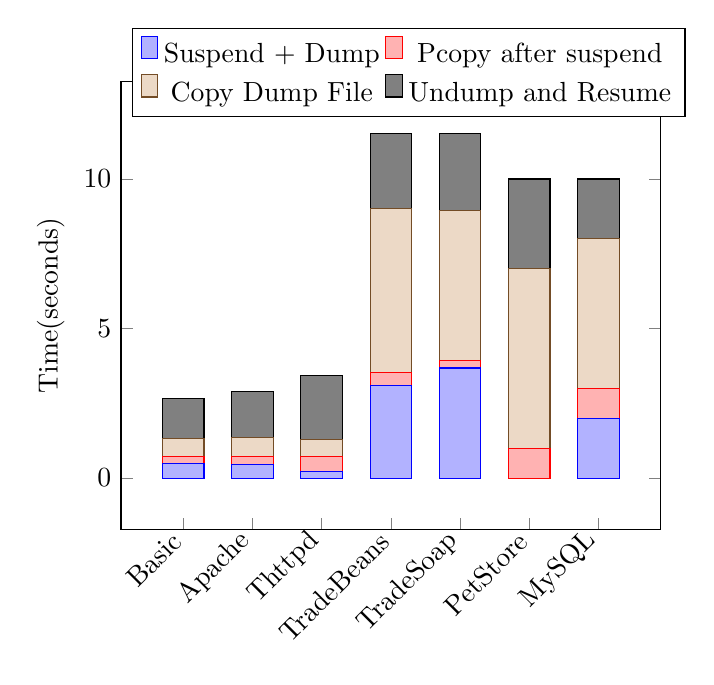
\begin{tikzpicture}
      \begin{axis}[
        ybar stacked,
        bar width=15pt,
        %	nodes near coords,
        enlargelimits=0.15,
        legend style={at={(0.02,1.12)},anchor=north west,legend columns=2},
        ylabel={Time(seconds)},
        symbolic x coords={Basic, Apache, Thttpd, TradeBeans, TradeSoap, 
          PetStore, MySQL},
        xtick=data,
        x tick label style={rotate=45,anchor=east},
        ]
        \addplot+[ybar] plot coordinates {(Basic,0.49) (Apache,0.46) (Thttpd,0.21) (TradeBeans,3.10) (TradeSoap,3.68) (PetStore,0) (MySQL,2) };
        \addplot+[ybar] plot coordinates {(Basic,0.22) (Apache,0.27) (Thttpd,0.50) (TradeBeans,0.44) (TradeSoap,0.25) (PetStore,1) (MySQL,1) };
        \addplot+[ybar] plot coordinates {(Basic,0.62) (Apache,0.64) (Thttpd,0.57) (TradeBeans,5.47) (TradeSoap,5.03) (PetStore,6) (MySQL,5) };
        \addplot+[ybar] plot coordinates {(Basic,1.33) (Apache,1.53) (Thttpd,2.14) (TradeBeans,2.51) (TradeSoap,2.57) (PetStore,3) (MySQL,2) };
        \addlegendentry{\strut Suspend + Dump}
        \addlegendentry{\strut Pcopy after suspend}
        \addlegendentry{\strut Copy Dump File}
        \addlegendentry{\strut Undump and Resume}
        %	\legend{\strut Suspend + Dump, \strut Pcopy after suspend, \strut Copy Dump File, \strut Undump and Resume}
      \end{axis}
    \end{tikzpicture}
  }
  \captionsetup{justification=centering}
  \caption{Suspend time for live cloning, when running a representative benchmark}
  \label{fig:stats}
\end{figure}


Overall we conclude, that "live cloning" takes only a few seconds (~2/3 secs) and is not disruptive to application clients (there is no loss of service visible). 
However, in high I/O write intensive workloads, the amount of time taken to clone can go up to a couple of mins (~3/4 mins).
In such cases, we did observe a few retries and in http but no timeouts, naturally the performance of the server did suffer. 
Current research in live migration has looked into further decreasing the sync time by doing active migration, and trigger page fault for the dirty bits which were not copied over.
This is a similar to a copy-on-write method, that could possibly reduce our suspend time.
In the interest of time, we have not explored faster means of live cloning, but aim to do so in our future work.
%However, it would impact, the overall performance of both systems as it would do the rsync operation for a much longer time-period.

\begin{table}[h]
\begin{centering}
\begin{tabular}{|c|c|c|c|}
\hline
\begin{tabular}[c]{@{}c@{}}Input \\ Rate\end{tabular}          & \begin{tabular}[c]{@{}c@{}}Debug\\ Window\end{tabular} & \begin{tabular}[c]{@{}c@{}}Pipe\\ Size\end{tabular} & Delay \\ \hline
530 bps, 27 rq/s                                               & N.A                                                    & 4096                                                & 2x    \\ \hline
530 bps, 27 rq/s                                               & 8sec                                                   & 4096                                                & 3x    \\ \hline
530 bps, 27 rq/s                                               & 72 sec                                                 & 16384                                               & 3x    \\ \hline
%\begin{tabular}[c]{@{}c@{}}Normal \\ Distribution\end{tabular} & 5 mins                                                 & 8192                                                & 2.5x  \\ \hline
%u Dist                                                         & N.A                                                    & 1M                                                  & 3.5x  \\ \hline
\end{tabular}
\caption{Approximate debug window sizes }
\label{table:timewindow}
\end{centering}
\end{table}

\subsection{Debug-Window Size Evaluation}
\label{sec:timewindowPerformance}

%As explained in section \ref{sec:timewindowPerformance} if the overhead of the test-container is too high, the buffer may overflow.
%This indirectly means that the test-container and the production-container are potentially out of sync.
We call the time taken to reach a buffer overflow the ``debug-window'' for the debug-container.
As explained earlier(see section \ref{sec:timewindowPerformance}, the size of this debug-window, depends both on the overhead of the ``instrumentation'', the incoming workload distribution and the size of the buffer.
In table \ref{table:timewindow}, we show the ``debug-window'' size for a fixed rate input to a MySQL server. 
The server is essentially getting select queries at a rate of 582 bps, we induce approximately a 2-4x slowdown, to get an idea of debug-window sizes. 
The slowdown is generated by first finding the average bandwidth of the MySQL server, and then putting a sleep to approximately model the overhead.
The entire experiment ran for about 6 mins each.
In general we found that for overheads upto 2x we experienced no buffer overflows, most function tracing and profiling tools generally have an overhead of 1-1.2x for lower granularity and 1.5-1.8x for higher granularity tracing.
For higher overheads the overflow depended on primarily the pipe-size, but with a 1M pipe we were able to sustain the window for several minutes as typically the size of MySQL requests are small.

We also tried a gaussian request distribution with request interarrival time being randomized to exhibhit a bursty behavior with high utilization. 
We found that 
 
%In this section we evaluate the testing window size using varying amounts of instrumentation, and the workload.
%For the purpose of this evaluation, we keep a fixed buffer size. 
%First we use a controlled workload rate, and gradually increase the overhead, then we use another scenario, where we keep the try to keep the same overhead, and try to increase the workload.
%We also use real-world network packet capture data, to simulate a realistic workload and gradually increase the overhead there

%\texttt{Nipun's note: This section still needs to be completed, I'm finishing up some of the results, before I can generate the charts}

\iffalse
\subsection{Overhead while Running tests}
\label{sec:overhead}

One of the most important goals of using \parikshan is to allow debugging without having any overhead on the actual application.
In this section we verify that this goal of \parikshan holds true i.e. debugging in the sandbox-container, does not effect the performance container. 
To understand the effect we ran some tests on our cloned container, with an independent cpu hog (infinite while loop with sleep) running within the test.
We gradually increased the amount of cpu being used by the cpu hog and found that while in the external mode there is no effect on the performance of the production container, in the internal mode at higher cpu hog percentages, the throughput of the production container is reduced.
This was an expected result, as the production container and test-container time share resources on the same machine, whereas in the external mode, they are completely isolated.
However, it is to be noted, that most debugging scenarios are unlikely to be cpu hogs, and if resource management in the container level is done properly, the containers in the internal-mode can be largely isolated from each other.
\fi
	
%\begin{figure*}
%	\begin{subfigure}[b]{0.45\textwidth}
\begin{figure}
  % [b]{0.45\textwidth}
  \centering
  \resizebox{\linewidth}{!}{
    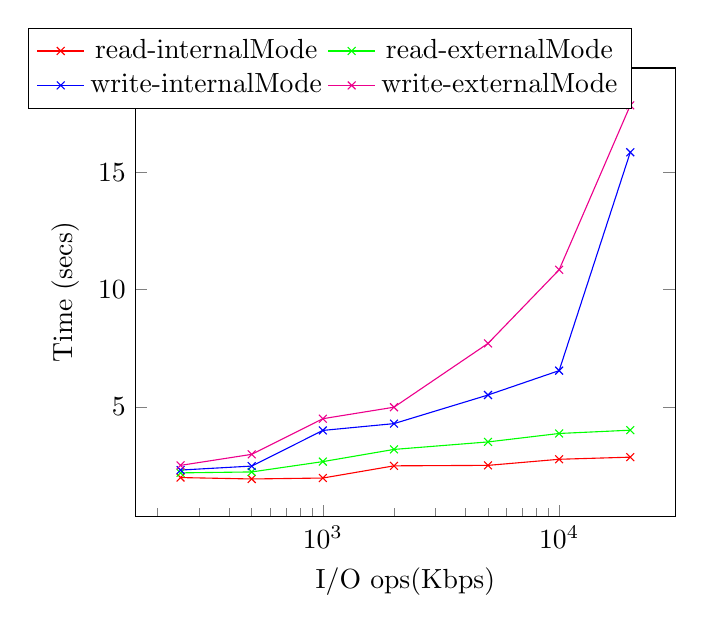
\begin{tikzpicture}
      \begin{axis}[
        xmode=log,
        legend style={at={(-0.2,1.09)},anchor=north west,legend columns=2},
        xlabel=I/O ops(Kbps),
        ylabel=Time (secs)]
        \addplot[color=red,mark=x] coordinates {
          (0,1.85)
          (250,1.99)
          (500,1.93)
          (1000,1.97)
          (2000,2.49)
          (5000,2.51)
          (10000,2.77)
          (20000,2.86)
        };
        \addlegendentry{read-internalMode}
        \addplot[color=green,mark=x] coordinates {
          (0,1.97)
          (250,2.19)
          (500,2.23)
          (1000,2.67)
          (2000,3.19)
          (5000,3.51)
          (10000,3.87)
          (20000,4.01)
        };
        \addlegendentry{read-externalMode}				
        \addplot[color=blue,mark=x] coordinates {
          (0,1.85)
          (250,2.31)
          (500,2.48)
          (1000,4.00)
          (2000,4.29)
          (5000,5.51)
          (10000,6.55)
          (20000,15.86)
        };
        \addlegendentry{write-internalMode}				
        \addplot[color=magenta,mark=x] coordinates {
          (0,1.87)
          (250,2.51)
          (500,2.98)
          (1000,4.50)
          (2000,4.99)
          (5000,7.71)
          (10000,10.85)
          (20000,17.86)
        };
        \addlegendentry{write-externalMode}
      \end{axis}
    \end{tikzpicture}
  }
  \captionsetup{justification=centering}
  \caption{Live Cloning suspend time whith increasing amounts of I/O operations }
  \label{fig:fioResults}
\end{figure}


\iffalse
In this section we present the evaluation of \parikshan. 
The key questions facing us were:
\begin{itemize}
%  \item How can \parikshan be used in the real world? 
%  \item Does the test container faithfully represent the execution and the state of the production container? 
   \item How does cloning the container effect the performance of the production container?
   \item How long of a testing-window do we have? 
   \item How does running tests in the test-container effect the performance of the production container?
\end{itemize}
In order to answer these questions, we separated our evaluation in looking at two different stages: cloning stage, time-window analysis.

\begin{table*}[ht]
  \centering
    \begin{tabular}{ | p{4cm} | l | l | l | l | l | l | l | l | l |}
    \hline
    \textbf{Modes} & \multicolumn{3}{|c|}{\textbf{Internal Mode}} & \multicolumn{3}{|c|}{\textbf{External Mode}} & \multicolumn{3}{|c|}{\textbf{Google Compute}}\\\hline
    \textbf{ } & \textbf{Cl} & \textbf{Hog} & \textbf{Hog+Cl} & \textbf{Cl} & \textbf{Hog} & \textbf{Hog+Cl} & \textbf{Cl} & \textbf{Hog} & \textbf{Hog+Cl} \\ \hline
    \hline
    \textbf{Throughput} & -- & 1691.0 req/s & 1509 req/s & -- & 712 & 625 & -- & 510 & 450\\ \hline
    \hline
    \textbf{Suspend + Dump} & 0.49 & -- & 0.46 & 0.10 & -- & 0.10 & 0.00 & 0.00 & 0.00\\ \hline
    \textbf{Pcopy after suspend} & 0.22 & -- & 0.27 & 0.44 & -- & 0.39 & 0.00 & 0.00 & 0.00\\ \hline
    \textbf{Copy Dump File} & 0.62 &  -- & 0.64 & 0.28 & -- & 0.31 & 0.67 & 0.00 & 0.00\\ \hline
    \textbf{Undump and Resume} & 1.33 &  -- & 1.53 & 0.84 & -- & 1.03 & 0.00 & 0.00 & 0.00\\ \hline 
    %\textbf{--------------} & --- & --- & --- & --- & --- & --- & --- & --- & --- \\ 
    \hline
    \textbf{Total Suspend Time} & 2.66 &  -- & 2.91 & 1.67 & -- & 1.83 & 0.00 & 0.00 & 0.00\\ \hline
    \end{tabular}
    \captionsetup{justification=centering}
	\caption{Performance of httpd throughput, and cloning time in external vs internal vs google compute modes}
	\label{table:clonePerf}
\end{table*}
\fi


\iffalse
The first column gives the average performance of the cloning operation without any hog operation running on it.  
An idle or a container with minimal processing is cloned relatively fast ~ 2.66 seconds on the idle container. 
We then tried to run an apache hog to make a baseline of apache's performance without cloning, and found that a simple page fetch gave us a throughput of 1691 req/s (internal mode), and then we tried to do cloning of the same container while running the hog. and found negligible change in the cloning performance.
The key thing to note in these experiments for all 3 modes, was that we \textbf{did not have any connection failure or connection refused, and only a slight decline in the throughput during the cloning operation}. 
Naturally, at the application layer, the tcp packet drops are hidden as packet resends from within tcp protocol hides the performance impact.
To further investigate the tcp packet dropping, we ran an iperf\cite{iperf}( a tool to measure tcp benchmark) server while cloning the production container. 
We were indeed able to observe packet dropping for about 2 seconds in the iperf client, however, the important point to note is that there were no requests dropped for the application while doing cloning. 


\begin{figure*}[t]
	\begin{center}
		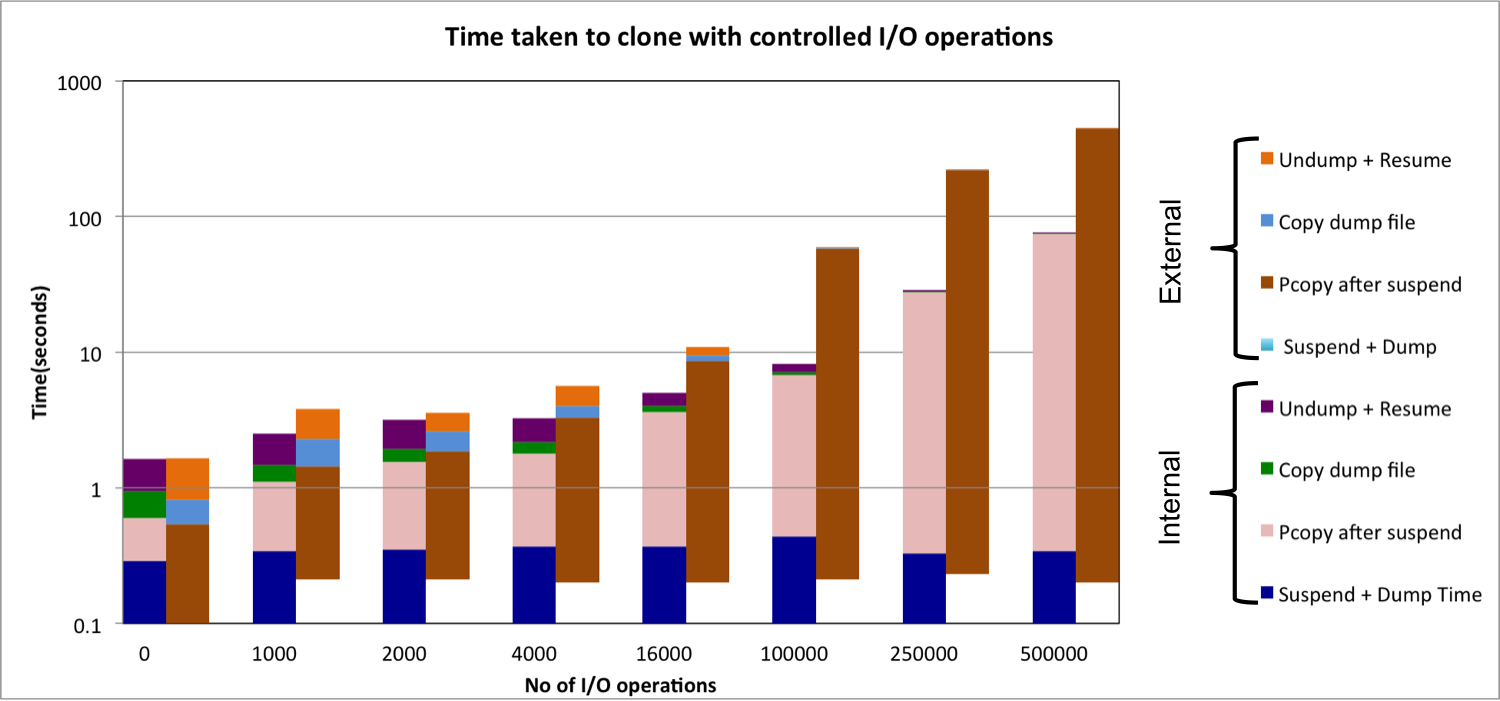
\includegraphics[width=1\textwidth]{figs/fioResult.png}
		\caption{Comparison between cloning between the internal vs external mode, while continuously increasing the file write operations to disk}
		\label{fig:fioResults}
	\end{center}
\end{figure*}
\fi
